\documentclass[a4paper,12pt]{beamer}

\usepackage{préambule}
\usetikzlibrary{calc,arrows.meta}
\usepackage{ifthen}

\newcommand{\mysize}{\scriptsize}
\newcommand{\mysizebis}{\tiny}
\newcommand{\myarrow}{{Latex[length=1mm, width=1mm]}-{Latex[length=1mm, width=1mm]}}
\newcommand{\affichecorrection}{1}

\newcommand{\correction}[1]{
	\ifthenelse{\affichecorrection=1}{{\color{red}#1}}{. . . . . .}
}

\begin{document}

\begin{frame}
	\frametitle{Exercice}

	Pour chaque segment, \textbf{reproduit le sur ton cahier}, puis écrit une expression pour sa longueur, en simplifiant le plus possible : \vspace{0.5cm}

	\begin{tabular}{cc}
		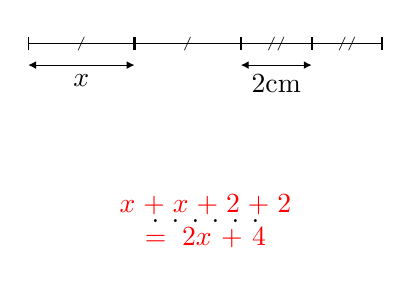
\begin{tikzpicture}[scale=0.9]
			\coordinate (P1) at (0,0);
			\coordinate (P2) at (1.5,0);
			\coordinate (P3) at (3,0);
			\coordinate (P4) at (4,0);
			\coordinate (P5) at (5,0);

			\draw[|-|] (P1) -- node{\mysizebis /} (P2);
			\draw[|-|] (P2) -- node{\mysizebis /} (P3);
			\draw[|-|] (P3) -- node{\mysizebis //} (P4);
			\draw[|-|] (P4) -- node{\mysizebis //} (P5);

			\draw[\myarrow] ($(P1) - (0,0.3)$) -- node[below] {$x$} ($(P2) - (0,0.3)$);

			\draw[\myarrow] ($(P3) - (0,0.3)$) -- node[below] {2cm} ($(P4) - (0,0.3)$);

			\node<1> at (2.5,-2.5) {. . . . . .};
			\ifthenelse{\affichecorrection=1}{
				\node<2>[text width=3cm,align=center] at (2.5,-2.5) {\correction{$x + x + 2 + 2$\\$= 2x + 4$}};
			}{}
		\end{tikzpicture} & \hspace{0.7cm} 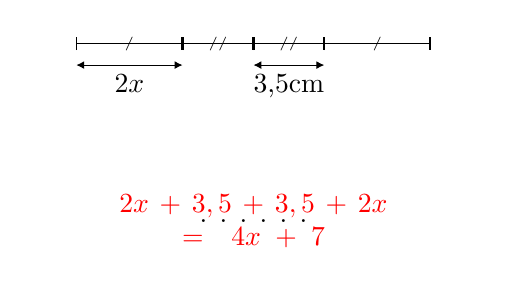
\begin{tikzpicture}[scale=0.9]
			\coordinate (P1) at (0,0);
			\coordinate (P2) at (1.5,0);
			\coordinate (P3) at (2.5,0);
			\coordinate (P4) at (3.5,0);
			\coordinate (P5) at (5,0);

			\draw[|-|] (P1) -- node{\mysizebis /} (P2);
			\draw[|-|] (P2) -- node{\mysizebis //} (P3);
			\draw[|-|] (P3) -- node{\mysizebis //} (P4);
			\draw[|-|] (P4) -- node{\mysizebis /} (P5);

			\draw[\myarrow] ($(P1) - (0,0.3)$) -- node[below] {$2×x$} ($(P2) - (0,0.3)$);

			\draw[\myarrow] ($(P3) - (0,0.3)$) -- node[below] {3,5cm} ($(P4) - (0,0.3)$);

			\node<1> at (2.5,-2.5) {. . . . . .};
			\ifthenelse{\affichecorrection=1}{
				\node<2>[text width=5.5cm,align=center] at (2.5,-2.5) {\correction{$2×x + 3,5 + 3,5 + 2×x$\\$= 4x + 7$}};
			}{}
		\end{tikzpicture}
	\end{tabular}
\end{frame}

\begin{frame}
	\frametitle{Exercice}

	Pour chaque figure, \textbf{la reproduire} puis écrire son périmètre en simplifiant le plus possible :

	\begin{tabular}{cc}
		\begin{tikzpicture}
			\newcommand*{\x}{2};
			\newcommand*{\y}{2.5};

			\draw (0,0)
			-- node{\mysize //} ++(\x,0)
			-- node{\mysize /} ++(0,\y)
			-- node{\mysize //} ++(-\x,0)
			-- node{\mysize /} cycle;

			\draw[\myarrow] (0,-0.3) -- node[below] {\small $x$} ++(\x,0);
			\draw[\myarrow] (-0.3,0) -- node[left] {\small $2{,}5$cm} ++(0,\y);

			\node<1> at (\x / 2,-2) {. . . . . .};
			\ifthenelse{\affichecorrection=1}{
				\node<2>[text width=4cm,align=center] at (\x / 2,-2) {\correction{$x + 2,5 + x + 2,5$\\ $= 2x + 5$}};
			}{}
		\end{tikzpicture} & 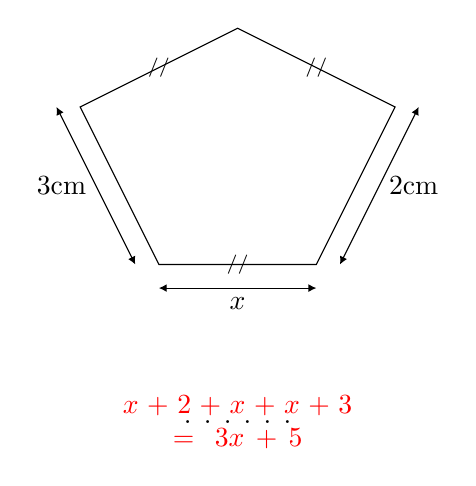
\begin{tikzpicture}
			\coordinate (P1) at (0,0);
			\coordinate (P2) at (2,0);
			\coordinate (P3) at (3,2);
			\coordinate (P4) at (1,3);
			\coordinate (P5) at (-1,2);

			\draw (P1)
			-- node{\mysize //} (P2)
			-- (P3)
			-- node{\mysize //} (P4)
			-- node{\mysize //} (P5)
			-- cycle;

			\draw[\myarrow] ($(P1) - (0,0.3)$) -- node[below] {$x$} ($(P2) - (0,0.3)$);

			\draw[\myarrow] ($(P5) - (0.3,0)$) -- node[left] {3cm} ($(P1) - (0.3,0)$);
			\draw[\myarrow] ($(P2) + (0.3,0)$) -- node[right] {2cm} ($(P3) + (0.3,0)$);

			\node<1> at (1,-2) {. . . . . .};
			\ifthenelse{\affichecorrection=1}{
				\node<2>[text width=4cm,align=center] at (1,-2) {\correction{$x + 2 + x + x + 3$\\ $= 3x + 5$}};
			}{}
		\end{tikzpicture}
	\end{tabular}
\end{frame}

\begin{frame}
	\frametitle{Exercice}

	Simplifie les expressions suivantes :

	\only<1> {
		\begin{itemize}
			\setlength\itemsep{1em}
			\item $0×x + 5 + 2×x =$ \dotfill
			\item $4×x + 3×4 =$ \dotfill
			\item $5×x + 1 + 2×x + 3 =$ \dotfill
			\item $0×x + 1×x + 2×y - 2×y =$ \dotfill
			\item $2{,}5×x - (2 + 1{,}5×x) + 2 =$ \dotfill
		\end{itemize}
	}

	\ifthenelse{\affichecorrection=1}{
		\only<2> {
			\begin{itemize}
				\setlength\itemsep{1em}
				\item $0×x + 5 + 2×x =$ \correction{$2x + 5$}
				\item $4×x + 3×4 =$ \correction{$4x + 12$}
				\item $5×x + 1 + 2×x + 3 =$ \correction{$5x + 1 + 2x + 3 = 7x + 4$}
				\item $0×x + 1×x + 2×y - 2×y =$ \correction{$0x + 1x + 2y - 2y = x$}
				\item $2{,}5×x - (2 + 1{,}5×x) + 2 =$ \correction{$2,5x - 2 - 1,5x + 2 = x$}
			\end{itemize}
		}
	}{}
\end{frame}

\end{document}